% Options for packages loaded elsewhere
\PassOptionsToPackage{unicode}{hyperref}
\PassOptionsToPackage{hyphens}{url}
\documentclass[
]{article}
\usepackage{xcolor}
\usepackage{amsmath,amssymb}
\setcounter{secnumdepth}{-\maxdimen} % remove section numbering
\usepackage{iftex}
\ifPDFTeX
  \usepackage[T1]{fontenc}
  \usepackage[utf8]{inputenc}
  \usepackage{textcomp} % provide euro and other symbols
\else % if luatex or xetex
  \usepackage{unicode-math} % this also loads fontspec
  \defaultfontfeatures{Scale=MatchLowercase}
  \defaultfontfeatures[\rmfamily]{Ligatures=TeX,Scale=1}
\fi
\usepackage{lmodern}
\ifPDFTeX\else
  % xetex/luatex font selection
\fi
% Use upquote if available, for straight quotes in verbatim environments
\IfFileExists{upquote.sty}{\usepackage{upquote}}{}
\IfFileExists{microtype.sty}{% use microtype if available
  \usepackage[]{microtype}
  \UseMicrotypeSet[protrusion]{basicmath} % disable protrusion for tt fonts
}{}
\makeatletter
\@ifundefined{KOMAClassName}{% if non-KOMA class
  \IfFileExists{parskip.sty}{%
    \usepackage{parskip}
  }{% else
    \setlength{\parindent}{0pt}
    \setlength{\parskip}{6pt plus 2pt minus 1pt}}
}{% if KOMA class
  \KOMAoptions{parskip=half}}
\makeatother
\usepackage{color}
\usepackage{fancyvrb}
\newcommand{\VerbBar}{|}
\newcommand{\VERB}{\Verb[commandchars=\\\{\}]}
\DefineVerbatimEnvironment{Highlighting}{Verbatim}{commandchars=\\\{\}}
% Add ',fontsize=\small' for more characters per line
\newenvironment{Shaded}{}{}
\newcommand{\AlertTok}[1]{\textcolor[rgb]{1.00,0.00,0.00}{\textbf{#1}}}
\newcommand{\AnnotationTok}[1]{\textcolor[rgb]{0.38,0.63,0.69}{\textbf{\textit{#1}}}}
\newcommand{\AttributeTok}[1]{\textcolor[rgb]{0.49,0.56,0.16}{#1}}
\newcommand{\BaseNTok}[1]{\textcolor[rgb]{0.25,0.63,0.44}{#1}}
\newcommand{\BuiltInTok}[1]{\textcolor[rgb]{0.00,0.50,0.00}{#1}}
\newcommand{\CharTok}[1]{\textcolor[rgb]{0.25,0.44,0.63}{#1}}
\newcommand{\CommentTok}[1]{\textcolor[rgb]{0.38,0.63,0.69}{\textit{#1}}}
\newcommand{\CommentVarTok}[1]{\textcolor[rgb]{0.38,0.63,0.69}{\textbf{\textit{#1}}}}
\newcommand{\ConstantTok}[1]{\textcolor[rgb]{0.53,0.00,0.00}{#1}}
\newcommand{\ControlFlowTok}[1]{\textcolor[rgb]{0.00,0.44,0.13}{\textbf{#1}}}
\newcommand{\DataTypeTok}[1]{\textcolor[rgb]{0.56,0.13,0.00}{#1}}
\newcommand{\DecValTok}[1]{\textcolor[rgb]{0.25,0.63,0.44}{#1}}
\newcommand{\DocumentationTok}[1]{\textcolor[rgb]{0.73,0.13,0.13}{\textit{#1}}}
\newcommand{\ErrorTok}[1]{\textcolor[rgb]{1.00,0.00,0.00}{\textbf{#1}}}
\newcommand{\ExtensionTok}[1]{#1}
\newcommand{\FloatTok}[1]{\textcolor[rgb]{0.25,0.63,0.44}{#1}}
\newcommand{\FunctionTok}[1]{\textcolor[rgb]{0.02,0.16,0.49}{#1}}
\newcommand{\ImportTok}[1]{\textcolor[rgb]{0.00,0.50,0.00}{\textbf{#1}}}
\newcommand{\InformationTok}[1]{\textcolor[rgb]{0.38,0.63,0.69}{\textbf{\textit{#1}}}}
\newcommand{\KeywordTok}[1]{\textcolor[rgb]{0.00,0.44,0.13}{\textbf{#1}}}
\newcommand{\NormalTok}[1]{#1}
\newcommand{\OperatorTok}[1]{\textcolor[rgb]{0.40,0.40,0.40}{#1}}
\newcommand{\OtherTok}[1]{\textcolor[rgb]{0.00,0.44,0.13}{#1}}
\newcommand{\PreprocessorTok}[1]{\textcolor[rgb]{0.74,0.48,0.00}{#1}}
\newcommand{\RegionMarkerTok}[1]{#1}
\newcommand{\SpecialCharTok}[1]{\textcolor[rgb]{0.25,0.44,0.63}{#1}}
\newcommand{\SpecialStringTok}[1]{\textcolor[rgb]{0.73,0.40,0.53}{#1}}
\newcommand{\StringTok}[1]{\textcolor[rgb]{0.25,0.44,0.63}{#1}}
\newcommand{\VariableTok}[1]{\textcolor[rgb]{0.10,0.09,0.49}{#1}}
\newcommand{\VerbatimStringTok}[1]{\textcolor[rgb]{0.25,0.44,0.63}{#1}}
\newcommand{\WarningTok}[1]{\textcolor[rgb]{0.38,0.63,0.69}{\textbf{\textit{#1}}}}
\usepackage{longtable,booktabs,array}
\usepackage{calc} % for calculating minipage widths
% Correct order of tables after \paragraph or \subparagraph
\usepackage{etoolbox}
\makeatletter
\patchcmd\longtable{\par}{\if@noskipsec\mbox{}\fi\par}{}{}
\makeatother
% Allow footnotes in longtable head/foot
\IfFileExists{footnotehyper.sty}{\usepackage{footnotehyper}}{\usepackage{footnote}}
\makesavenoteenv{longtable}
\usepackage{graphicx}
\makeatletter
\newsavebox\pandoc@box
\newcommand*\pandocbounded[1]{% scales image to fit in text height/width
  \sbox\pandoc@box{#1}%
  \Gscale@div\@tempa{\textheight}{\dimexpr\ht\pandoc@box+\dp\pandoc@box\relax}%
  \Gscale@div\@tempb{\linewidth}{\wd\pandoc@box}%
  \ifdim\@tempb\p@<\@tempa\p@\let\@tempa\@tempb\fi% select the smaller of both
  \ifdim\@tempa\p@<\p@\scalebox{\@tempa}{\usebox\pandoc@box}%
  \else\usebox{\pandoc@box}%
  \fi%
}
% Set default figure placement to htbp
\def\fps@figure{htbp}
\makeatother
% definitions for citeproc citations
\NewDocumentCommand\citeproctext{}{}
\NewDocumentCommand\citeproc{mm}{%
  \begingroup\def\citeproctext{#2}\cite{#1}\endgroup}
\makeatletter
 % allow citations to break across lines
 \let\@cite@ofmt\@firstofone
 % avoid brackets around text for \cite:
 \def\@biblabel#1{}
 \def\@cite#1#2{{#1\if@tempswa , #2\fi}}
\makeatother
\newlength{\cslhangindent}
\setlength{\cslhangindent}{1.5em}
\newlength{\csllabelwidth}
\setlength{\csllabelwidth}{3em}
\newenvironment{CSLReferences}[2] % #1 hanging-indent, #2 entry-spacing
 {\begin{list}{}{%
  \setlength{\itemindent}{0pt}
  \setlength{\leftmargin}{0pt}
  \setlength{\parsep}{0pt}
  % turn on hanging indent if param 1 is 1
  \ifodd #1
   \setlength{\leftmargin}{\cslhangindent}
   \setlength{\itemindent}{-1\cslhangindent}
  \fi
  % set entry spacing
  \setlength{\itemsep}{#2\baselineskip}}}
 {\end{list}}
\usepackage{calc}
\newcommand{\CSLBlock}[1]{\hfill\break\parbox[t]{\linewidth}{\strut\ignorespaces#1\strut}}
\newcommand{\CSLLeftMargin}[1]{\parbox[t]{\csllabelwidth}{\strut#1\strut}}
\newcommand{\CSLRightInline}[1]{\parbox[t]{\linewidth - \csllabelwidth}{\strut#1\strut}}
\newcommand{\CSLIndent}[1]{\hspace{\cslhangindent}#1}
\ifLuaTeX
\usepackage[bidi=basic]{babel}
\else
\usepackage[bidi=default]{babel}
\fi
\babelprovide[main,import]{french}
% get rid of language-specific shorthands (see #6817):
\let\LanguageShortHands\languageshorthands
\def\languageshorthands#1{}
\setlength{\emergencystretch}{3em} % prevent overfull lines
\providecommand{\tightlist}{%
  \setlength{\itemsep}{0pt}\setlength{\parskip}{0pt}}
\usepackage{bookmark}
\IfFileExists{xurl.sty}{\usepackage{xurl}}{} % add URL line breaks if available
\urlstyle{same}
\hypersetup{
  pdftitle={2~ Importation et manipulation de données spatiales -- Traitement d\textquotesingle images satellites avec Python},
  pdflang={fr},
  hidelinks,
  pdfcreator={LaTeX via pandoc}}

\title{2~ Importation et manipulation de données spatiales -- Traitement
d\textquotesingle images satellites avec Python}
\author{}
\date{}

\begin{document}
\maketitle

\phantomsection\label{quarto-document-content}
\phantomsection\label{title-block-header}
\section{\texorpdfstring{\protect\hypertarget{sec-chap01}{}{{2}~
{Importation et manipulation de données
spatiales}}}{2~ Importation et manipulation de données spatiales}}\label{importation-et-manipulation-de-donnuxe9es-spatiales}

\subsection{\texorpdfstring{{2.1}
Préambule}{2.1 Préambule}}\label{pruxe9ambule}

Assurez-vous de lire ce préambule avant d'exécutez le reste du notebook.
\#\#\# Objectifs Dans ce chapitre, nous abordons quelques formats
d'images ainsi que leur lecture. Ce chapitre est aussi disponible sous
la forme d'un notebook Python:

\href{https://colab.research.google.com/github/sfoucher/TraitementImagesPythonVol1/blob/main/notebooks/01-ImportationManipulationImages.ipynb}{\pandocbounded{
\includegraphics[keepaspectratio]{images/colab.png}}}

\subsubsection{\texorpdfstring{{2.1.1}
Librairies}{2.1.1 Librairies}}\label{librairies}

Les librairies qui vont être explorées dans ce chapitre sont les
suivantes:

\begin{itemize}
\item
  \href{https://scipy.org/}{SciPy}
\item
  \href{https://numpy.org/}{NumPy}
\item
  \href{https://pypi.org/project/opencv-python/}{opencv-python · PyPI}
\item
  \href{https://scikit-image.org/}{scikit-image}
\item
  \href{https://rasterio.readthedocs.io/en/stable/}{Rasterio}
\item
  \href{https://docs.xarray.dev/en/stable/}{Xarray}
\item
  \href{https://corteva.github.io/rioxarray/stable/index.html}{rioxarray}
\end{itemize}

Dans l'environnement Google Colab, seul \texttt{rioxarray} et gdal
doivent être installé:

\phantomsection\label{7e7dc626}
\phantomsection\label{cb1}
\begin{Shaded}
\begin{Highlighting}[]
\OperatorTok{!}\NormalTok{apt}\OperatorTok{{-}}\NormalTok{get update}
\OperatorTok{!}\NormalTok{apt}\OperatorTok{{-}}\NormalTok{get install gdal}\OperatorTok{{-}}\BuiltInTok{bin}\NormalTok{ libgdal}\OperatorTok{{-}}\NormalTok{dev}
\OperatorTok{!}\NormalTok{pip install }\OperatorTok{{-}}\NormalTok{q rioxarray}
\end{Highlighting}
\end{Shaded}

Vérifier les importations:

\phantomsection\label{5683ceab}
\phantomsection\label{cb2}
\begin{Shaded}
\begin{Highlighting}[]
\ImportTok{import}\NormalTok{ numpy }\ImportTok{as}\NormalTok{ np}
\ImportTok{import}\NormalTok{ rioxarray }\ImportTok{as}\NormalTok{ rxr}
\ImportTok{from}\NormalTok{ scipy }\ImportTok{import}\NormalTok{ signal}
\ImportTok{import}\NormalTok{ xarray }\ImportTok{as}\NormalTok{ xr}
\ImportTok{import}\NormalTok{ xrscipy}
\ImportTok{import}\NormalTok{ matplotlib.pyplot }\ImportTok{as}\NormalTok{ plt}
\end{Highlighting}
\end{Shaded}

\subsubsection{\texorpdfstring{{2.1.2}
Données}{2.1.2 Données}}\label{donnuxe9es}

Nous allons utilisés ces images dans ce chapitre:

\phantomsection\label{a0e83a09}
\phantomsection\label{cb3}
\begin{Shaded}
\begin{Highlighting}[]
\ImportTok{import}\NormalTok{ gdown}

\NormalTok{gdown.download(}\StringTok{\textquotesingle{}https://drive.google.com/uc?export=download\&confirm=pbef\&id=1a6Ypg0g1Oy4AJt9XWKWfnR12NW1XhNg\_\textquotesingle{}}\NormalTok{, output}\OperatorTok{=} \StringTok{\textquotesingle{}RGBNIR\_of\_S2A.tif\textquotesingle{}}\NormalTok{)}
\NormalTok{gdown.download(}\StringTok{\textquotesingle{}https://drive.google.com/uc?export=download\&confirm=pbef\&id=1a4PQ68Ru8zBphbQ22j0sgJ4D2quw{-}Wo6\textquotesingle{}}\NormalTok{, output}\OperatorTok{=} \StringTok{\textquotesingle{}landsat7.tif\textquotesingle{}}\NormalTok{)}
\NormalTok{gdown.download(}\StringTok{\textquotesingle{}https://drive.google.com/uc?export=download\&confirm=pbef\&id=1\_zwCLN{-}x7XJcNHJCH6Z8upEdUXtVtvs1\textquotesingle{}}\NormalTok{, output}\OperatorTok{=} \StringTok{\textquotesingle{}berkeley.jpg\textquotesingle{}}\NormalTok{)}
\OperatorTok{!}\NormalTok{wget https:}\OperatorTok{//}\NormalTok{raw.githubusercontent.com}\OperatorTok{/}\NormalTok{sfoucher}\OperatorTok{/}\NormalTok{TraitementImagesPythonVol1}\OperatorTok{/}\NormalTok{refs}\OperatorTok{/}\NormalTok{heads}\OperatorTok{/}\NormalTok{main}\OperatorTok{/}\NormalTok{images}\OperatorTok{/}\NormalTok{modis}\OperatorTok{{-}}\NormalTok{aqua.PNG }\OperatorTok{{-}}\NormalTok{O modis}\OperatorTok{{-}}\NormalTok{aqua.PNG}
\end{Highlighting}
\end{Shaded}

Vérifiez que vous êtes capable de les lire :

\phantomsection\label{6ff6fd43}
\phantomsection\label{cb4}
\begin{Shaded}
\begin{Highlighting}[]
\ControlFlowTok{with}\NormalTok{ rxr.open\_rasterio(}\StringTok{\textquotesingle{}berkeley.jpg\textquotesingle{}}\NormalTok{, mask\_and\_scale}\OperatorTok{=} \VariableTok{True}\NormalTok{) }\ImportTok{as}\NormalTok{ img\_rgb:}
    \BuiltInTok{print}\NormalTok{(img\_rgb)}
\ControlFlowTok{with}\NormalTok{ rxr.open\_rasterio(}\StringTok{\textquotesingle{}RGBNIR\_of\_S2A.tif\textquotesingle{}}\NormalTok{, mask\_and\_scale}\OperatorTok{=} \VariableTok{True}\NormalTok{) }\ImportTok{as}\NormalTok{ img\_rgbnir:}
    \BuiltInTok{print}\NormalTok{(img\_rgbnir)}
\end{Highlighting}
\end{Shaded}

\subsection{\texorpdfstring{{2.2} Importation
d'images}{2.2 Importation d'images}}\label{importation-dimages}

La première étape avant tout traitement est d'accéder à la donnée image
pour qu'elle soit manipulée par le langage Python. L'imagerie satellite
présente certains défis notamment en raison de la taille parfois très
importante des images. Il existe maintenant certaines librairies, comme
\href{https://docs.xarray.dev/en/stable/}{Xarray}, qui on cherchées à
optimiser la lecture et l'écriture de grandes images. Il est donc
conseiller de toujours garder un oeil sur l'espace mémoire occupé par
les variables Python représentant les images. La librairie principale en
géomatique qui va nous permettre d'importer (et d'exporter) de
l'imagerie est la librairie \href{https://gdal.org}{GDAL} qui rassemble
la plupart des formats sous forme de \emph{driver} (ou pilote en
français).

Dans le domaine de la géomatique, il faut prêter attention à trois
caractéristiques principales des images: 1. \textbf{La matrice des
données} elle-même qui contient les valeurs brutes des pixels. Cette
matrice sera souvent un cube à trois dimensions. En Python, ce cube sera
le plus souvent un objet de la librairie
\href{https://numpy.org/}{NumPy} (voir section). 2. \textbf{La dynamique
des images} c.à.d le format de stockage des valeurs individuelles
(octet, entier, double, etc.). Ce format décide principalement de la
résolution radiométrique et des valeurs minimales et maximales
supportées. 3. \textbf{Le nombre de bandes} spectrales de l'image qui
est souvent supérieur à 3 et peut atteindre plusieurs centaines de
bandes pour certains capteurs. 4. \textbf{La métadonnée} qui va
transporter l'information auxiliaire de l'image comme les dimensions et
la position de l'image, la date, etc. Cette donnée auxiliaire prendra
souvent la forme d'un dictionnaire Python. Elle contiendra aussi
l'information de géoréférence.

Les différents formats se distinguent principalement sur la manière dont
ces trois caractéristiques sont gérées.

\subsubsection{\texorpdfstring{{2.2.1} Formats des
images}{2.2.1 Formats des images}}\label{formats-des-images}

Il existe maintenant de nombreux formats numériques pour la donnée de
type image parfois appelé donnée matricielle ou donnée \emph{raster}. La
librairie GDAL rassemble la plupart des formats matriciels rencontrés en
géomatique (voir
\href{https://gdal.org/en/latest/drivers/raster/index.html}{Raster
drivers --- GDAL documentation} pour une liste complète).

On peut distinguer deux grandes familles de format: 1. Les formats de
type \textbf{RVB} issus de l'imagerie numérique grand publique comme
\href{https://gdal.org/en/latest/drivers/raster/jpeg.html\#raster-jpeg}{JPEG},
\href{https://gdal.org/en/latest/drivers/raster/png.html\#raster-png}{png},
etc. Ces formats ne supportent généralement que trois bandes au maximum
(rouge, vert et bleu) et des valeurs de niveaux de gris entre 0 et 255
(format dit 8 bit ou \texttt{uint8}). 2. \textbf{Les géo-formats} issus
des domaines scientifiques ou techniques comme GeoTIFF, HDF5, NetCDF,
etc. qui peuvent inclure plus que trois bandes et des dynamiques plus
élevées (16 bit ou même float).

Les formats RVB restent très utilisés en Python notamment par les
librairies dites de vision par ordinateur (\emph{Computer Vision}) comme
OpenCV et sickit-image ainsi que les grandes librairies en apprentissage
profond (PyTorch, Tensorflow).

\textbf{Installation de gdal dans un système Linux}

\begin{itemize}
\tightlist
\item
  Pour installer GDAL~:
\end{itemize}

\begin{verbatim}
!apt-get update
!apt-get install gdal-bin libgdal-dev
\end{verbatim}

\paragraph{\texorpdfstring{{2.2.1.1} Formats de type
RVB}{2.2.1.1 Formats de type RVB}}\label{formats-de-type-rvb}

Les premiers formats pour de l'imagerie à une bande (monochrome) et à
trois bandes (image couleur rouge-vert-bleu) sont issus du domaine des
sciences de l'ordinateur. On trouvera, entre autres, les formats pbm,
png et jpeg. Ces formats supportent peu de métadonnées et sont placées
dans un entête (\emph{header}) très limité. Cependant, ces formats
restent très populaires dans le domaine de la vision par ordinateur et
sont très utilisés en apprentissage profond en particulier. Pour la
lecture des images RVB, on peut utiliser les librairies Rasterio,
\href{https://he-arc.github.io/livre-python/pillow/index.html}{PIL} ou
\href{https://docs.opencv.org/4.10.0/index.html}{OpenCV}.

\subparagraph{\texorpdfstring{{2.2.1.1.1} Lecture avec la librairie
PIL}{2.2.1.1.1 Lecture avec la librairie PIL}}\label{lecture-avec-la-librairie-pil}

La librairie PIL retourne un objet de type \texttt{PngImageFile},
l'affichage de l'image se fait directement dans la cellule de sortie.

\phantomsection\label{4b67521d}
\phantomsection\label{lst-lecture-PIL-PNG}
\begin{figure}
\centering
\phantomsection\label{lst-lecture-PIL-PNG}
\begin{Shaded}
\begin{Highlighting}[]
\ImportTok{from}\NormalTok{ PIL }\ImportTok{import}\NormalTok{ Image}
\NormalTok{img }\OperatorTok{=}\NormalTok{ Image.}\BuiltInTok{open}\NormalTok{(}\StringTok{\textquotesingle{}modis{-}aqua.PNG\textquotesingle{}}\NormalTok{)}
\NormalTok{img}
\end{Highlighting}
\end{Shaded}
\caption{Bloc de code~2.1: Lecture d'une image en format PNG avec PIL}
\end{figure}

\begin{figure}
\centering
\pandocbounded{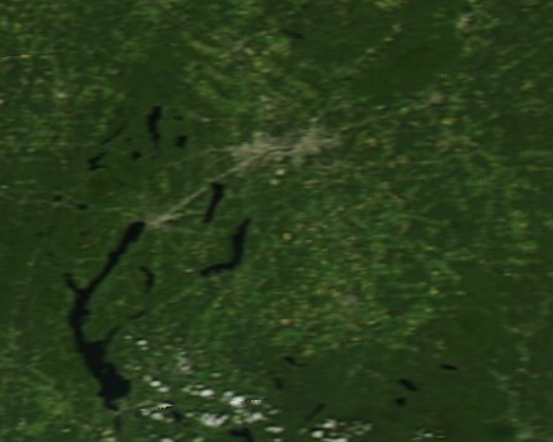
\includegraphics[keepaspectratio]{01-ImportationManipulationImages_files/figure-html/cell-6-output-1.png}}
\caption{}
\end{figure}

\subparagraph{\texorpdfstring{{2.2.1.1.2} Lecture avec la librairie
OpenCV}{2.2.1.1.2 Lecture avec la librairie OpenCV}}\label{lecture-avec-la-librairie-opencv}

La librairie \href{https://docs.opencv.org/4.10.0/index.html}{OpenCV}
est aussi très populaire en vision par ordinateur. La fonction
\texttt{imread} donne directement un objet de type NumPy en sortie.

\phantomsection\label{74707292}
\phantomsection\label{lst-lecture-opencv-PNG}
\begin{figure}
\centering
\phantomsection\label{lst-lecture-opencv-PNG}
\begin{Shaded}
\begin{Highlighting}[]
\ImportTok{import}\NormalTok{ cv2}
\NormalTok{img }\OperatorTok{=}\NormalTok{ cv2.imread(}\StringTok{\textquotesingle{}modis{-}aqua.PNG\textquotesingle{}}\NormalTok{)}
\NormalTok{img}
\end{Highlighting}
\end{Shaded}
\caption{Bloc de code~2.2: Lecture d'une image en format PNG avec
OpenCV}
\end{figure}

\begin{verbatim}
array([[[17, 50, 33],
        [15, 49, 31],
        [14, 48, 30],
        ...,
        [23, 56, 36],
        [23, 55, 36],
        [22, 55, 36]],

       [[18, 51, 34],
        [16, 50, 32],
        [15, 49, 32],
        ...,
        [27, 59, 40],
        [28, 60, 41],
        [27, 60, 41]],

       [[18, 53, 35],
        [18, 52, 34],
        [18, 51, 34],
        ...,
        [31, 64, 44],
        [34, 66, 47],
        [33, 65, 46]],

       ...,

       [[34, 74, 48],
        [35, 73, 48],
        [34, 70, 46],
        ...,
        [41, 74, 54],
        [41, 73, 54],
        [41, 73, 54]],

       [[36, 76, 50],
        [36, 74, 49],
        [35, 71, 47],
        ...,
        [37, 70, 51],
        [38, 71, 51],
        [38, 71, 51]],

       [[36, 76, 50],
        [35, 73, 48],
        [33, 69, 45],
        ...,
        [31, 63, 44],
        [33, 65, 46],
        [33, 66, 46]]], dtype=uint8)
\end{verbatim}

\subparagraph{\texorpdfstring{{2.2.1.1.3} Lecture avec la librairie
RasterIO}{2.2.1.1.3 Lecture avec la librairie RasterIO}}\label{lecture-avec-la-librairie-rasterio}

Rien ne nous empêche de lire une image de format RVB avec
\href{https://rasterio.readthedocs.io/en/stable/}{RasterIO} comme décrit
dans (\hyperref[lst-lecturerasterioPNG]{bloc~{2.3}}). Vous noterez
cependant les avertissements concernant l'absence de géoréférence pour
ce type d'image.

\phantomsection\label{26176f8f}
\phantomsection\label{lst-lecturerasterioPNG}
\begin{figure}
\centering
\phantomsection\label{lst-lecturerasterioPNG}
\begin{Shaded}
\begin{Highlighting}[]
\ImportTok{import}\NormalTok{ rasterio}
\NormalTok{img}\OperatorTok{=}\NormalTok{ rasterio.}\BuiltInTok{open}\NormalTok{(}\StringTok{\textquotesingle{}modis{-}aqua.PNG\textquotesingle{}}\NormalTok{)}
\NormalTok{img}
\end{Highlighting}
\end{Shaded}
\caption{Bloc de code~2.3: Lecture d'une image en format PNG avec
OpenCV}
\end{figure}

\begin{verbatim}
<open DatasetReader name='modis-aqua.PNG' mode='r'>
\end{verbatim}

\paragraph{\texorpdfstring{{2.2.1.2} Le format
GeoTiff}{2.2.1.2 Le format GeoTiff}}\label{le-format-geotiff}

Le format GeoTIFF est une extension du format TIFF (Tagged Image File
Format) qui permet d'incorporer des métadonnées géospatiales directement
dans un fichier image. Développé initialement par Dr.~Niles Ritter au
Jet Propulsion Laboratory de la
\href{https://www.earthdata.nasa.gov/esdis/esco/standards-and-practices/geotiff}{NASA}
dans les années 1990, GeoTIFF est devenu un standard de facto pour le
stockage et l'échange d'images géoréférencées dans les domaines de la
télédétection et des systèmes d'information géographique (SIG). Ce
format supporte plus que trois bandes aussi longtemps que ces bandes
sont de même dimension.

Le format GeoTIFF est très utilisé et est largement supporté par les
bibliothèques et logiciels géospatiaux, notamment
\href{https://gdal.org}{GDAL} (\emph{Geospatial Data Abstraction
Library}), qui offre des capacités de lecture et d'écriture pour ce
format. Cette compatibilité étendue a contribué à son adoption
généralisée dans la communauté géospatiale.

\subparagraph{\texorpdfstring{{2.2.1.2.1} Standardisation par
l'OGC}{2.2.1.2.1 Standardisation par l'OGC}}\label{standardisation-par-logc}

Le standard GeoTIFF proposé par l'Open Geospatial Consortium (OGC) en
2019 formalise et étend les spécifications originales du format GeoTIFF,
offrant une norme robuste pour l'échange d'images géoréférencées. Cette
standardisation, connue sous le nom d'OGC GeoTIFF 1.1
{(\href{references.html\#ref-OGCGeoTIFF}{2019})}, apporte plusieurs
améliorations et clarifications importantes.

\paragraph{\texorpdfstring{{2.2.1.3} Le format
COG}{2.2.1.3 Le format COG}}\label{le-format-cog}

Une innovation récente dans l'écosystème GeoTIFF est le format
\emph{Cloud Optimized GeoTIFF} (\href{http://cogeo.org/}{COG}), conçu
pour faciliter l'utilisation de fichiers GeoTIFF hébergés sur des
serveurs web HTTP. Le COG permet aux utilisateurs et aux logiciels
d'accéder à des parties spécifiques du fichier sans avoir à le
télécharger entièrement, ce qui est particulièrement utile pour les
applications basées sur le cloud.

\subsubsection{\texorpdfstring{{2.2.2} Métadonnées des
images}{2.2.2 Métadonnées des images}}\label{muxe9tadonnuxe9es-des-images}

La manière la plus directe d'accéder à la métadonnée d'une image est
d'utiliser les commandes
\href{https://rasterio.readthedocs.io/en/stable/cli.html\#info}{\texttt{rio\ info}}
de la librairie Rasterio ou \texttt{gdalinfo} de la librairie
\texttt{gdal}. Le résultat est imprimé dans la sortie standard ou sous
forme d'un dictionnaire Python.

\phantomsection\label{1b6d0b80}
\phantomsection\label{lst-gdalinfo}
\begin{figure}
\centering
\phantomsection\label{lst-gdalinfo}
\begin{Shaded}
\begin{Highlighting}[]
\OperatorTok{!}\NormalTok{gdalinfo RGBNIR\_of\_S2A.tif}
\end{Highlighting}
\end{Shaded}
\caption{Bloc de code~2.4: Collecte d'information sur une image avec
gdal}
\end{figure}

\begin{verbatim}
Warning 1: TIFFReadDirectory:Sum of Photometric type-related color channels and ExtraSamples doesn't match SamplesPerPixel. Defining non-color channels as ExtraSamples.
Driver: GTiff/GeoTIFF
Files: RGBNIR_of_S2A.tif
       RGBNIR_of_S2A.tif.aux.xml
Size is 2074, 1926
Coordinate System is:
PROJCS["WGS 84 / UTM zone 18N",
    GEOGCS["WGS 84",
        DATUM["WGS_1984",
            SPHEROID["WGS 84",6378137,298.257223563,
                AUTHORITY["EPSG","7030"]],
            AUTHORITY["EPSG","6326"]],
        PRIMEM["Greenwich",0,
            AUTHORITY["EPSG","8901"]],
        UNIT["degree",0.0174532925199433,
            AUTHORITY["EPSG","9122"]],
        AUTHORITY["EPSG","4326"]],
    PROJECTION["Transverse_Mercator"],
    PARAMETER["latitude_of_origin",0],
    PARAMETER["central_meridian",-75],
    PARAMETER["scale_factor",0.9996],
    PARAMETER["false_easting",500000],
    PARAMETER["false_northing",0],
    UNIT["metre",1,
        AUTHORITY["EPSG","9001"]],
    AXIS["Easting",EAST],
    AXIS["Northing",NORTH],
    AUTHORITY["EPSG","32618"]]
Origin = (731780.000000000000000,5040800.000000000000000)
Pixel Size = (10.000000000000000,-10.000000000000000)
Metadata:
  AREA_OR_POINT=Area
  TIFFTAG_IMAGEDESCRIPTION=subset_RGBNIR_of_S2A_MSIL2A_20240625T153941_N0510_R011_T18TYR_20240625T221903
  TIFFTAG_RESOLUTIONUNIT=1 (unitless)
  TIFFTAG_XRESOLUTION=1
  TIFFTAG_YRESOLUTION=1
Image Structure Metadata:
  INTERLEAVE=BAND
Corner Coordinates:
Upper Left  (  731780.000, 5040800.000) ( 72d 2' 3.11"W, 45d28'55.98"N)
Lower Left  (  731780.000, 5021540.000) ( 72d 2'35.69"W, 45d18'32.70"N)
Upper Right (  752520.000, 5040800.000) ( 71d46' 9.19"W, 45d28'30.08"N)
Lower Right (  752520.000, 5021540.000) ( 71d46'44.67"W, 45d18' 6.95"N)
Center      (  742150.000, 5031170.000) ( 71d54'23.16"W, 45d23'31.71"N)
Band 1 Block=2074x1926 Type=UInt16, ColorInterp=Gray
  Min=86.000 Max=15104.000 
  Minimum=86.000, Maximum=15104.000, Mean=1426.625, StdDev=306.564
  Metadata:
    STATISTICS_MAXIMUM=15104
    STATISTICS_MEAN=1426.6252674912
    STATISTICS_MINIMUM=86
    STATISTICS_STDDEV=306.56427126942
    STATISTICS_VALID_PERCENT=100
Band 2 Block=2074x1926 Type=UInt16, ColorInterp=Undefined
  Min=1139.000 Max=14352.000 
  Minimum=1139.000, Maximum=14352.000, Mean=1669.605, StdDev=310.919
  Metadata:
    STATISTICS_MAXIMUM=14352
    STATISTICS_MEAN=1669.6050060032
    STATISTICS_MINIMUM=1139
    STATISTICS_STDDEV=310.91935787639
    STATISTICS_VALID_PERCENT=100
Band 3 Block=2074x1926 Type=UInt16, ColorInterp=Undefined
  Min=706.000 Max=15280.000 
  Minimum=706.000, Maximum=15280.000, Mean=1471.392, StdDev=385.447
  Metadata:
    STATISTICS_MAXIMUM=15280
    STATISTICS_MEAN=1471.3923473736
    STATISTICS_MINIMUM=706
    STATISTICS_STDDEV=385.44654593014
    STATISTICS_VALID_PERCENT=100
Band 4 Block=2074x1926 Type=UInt16, ColorInterp=Undefined
  Min=1067.000 Max=15642.000 
  Minimum=1067.000, Maximum=15642.000, Mean=4393.945, StdDev=1037.934
  Metadata:
    STATISTICS_MAXIMUM=15642
    STATISTICS_MEAN=4393.94485025
    STATISTICS_MINIMUM=1067
    STATISTICS_STDDEV=1037.933939728
    STATISTICS_VALID_PERCENT=100
\end{verbatim}

Le plus simple est d'utiliser la fonction \texttt{rio\ info}:

\phantomsection\label{7c835ea3}
\phantomsection\label{lst-rioinfo}
\begin{figure}
\centering
\phantomsection\label{lst-rioinfo}
\begin{Shaded}
\begin{Highlighting}[]
\OperatorTok{!}\NormalTok{rio info RGBNIR\_of\_S2A.tif }\OperatorTok{{-}{-}}\NormalTok{indent }\DecValTok{2} \OperatorTok{{-}{-}}\NormalTok{verbose}
\end{Highlighting}
\end{Shaded}
\caption{Bloc de code~2.5: Collecte d'information sur une image avec
rasterio}
\end{figure}

\subsection{\texorpdfstring{{2.3} Manipulation des
images}{2.3 Manipulation des images}}\label{manipulation-des-images}

\subsubsection{\texorpdfstring{{2.3.1} Manipulation de la matrice de
pixels}{2.3.1 Manipulation de la matrice de pixels}}\label{manipulation-de-la-matrice-de-pixels}

La donnée brute de l'image est généralement contenue dans un cube
matricielle à trois dimensions (deux dimensions spatiales et une
dimension spectrale). Comme exposé précédemment, la librairie dite
\emph{``fondationnelle''} pour la manipulation de matrices en Python est
\href{https://numpy.org/}{NumPy}. Cette librairie contient un nombre
très important de fonctionnalités couvrant l'algèbre linéaires, les
statistiques, etc. et constitue la fondation de nombreuses librairies en
traitement numérique (voir (\hyperref[fig-naturenumpy1]{figure~{2.1}}))

\phantomsection\label{fig-naturenumpy1}
\begin{figure}
\centering
\pandocbounded{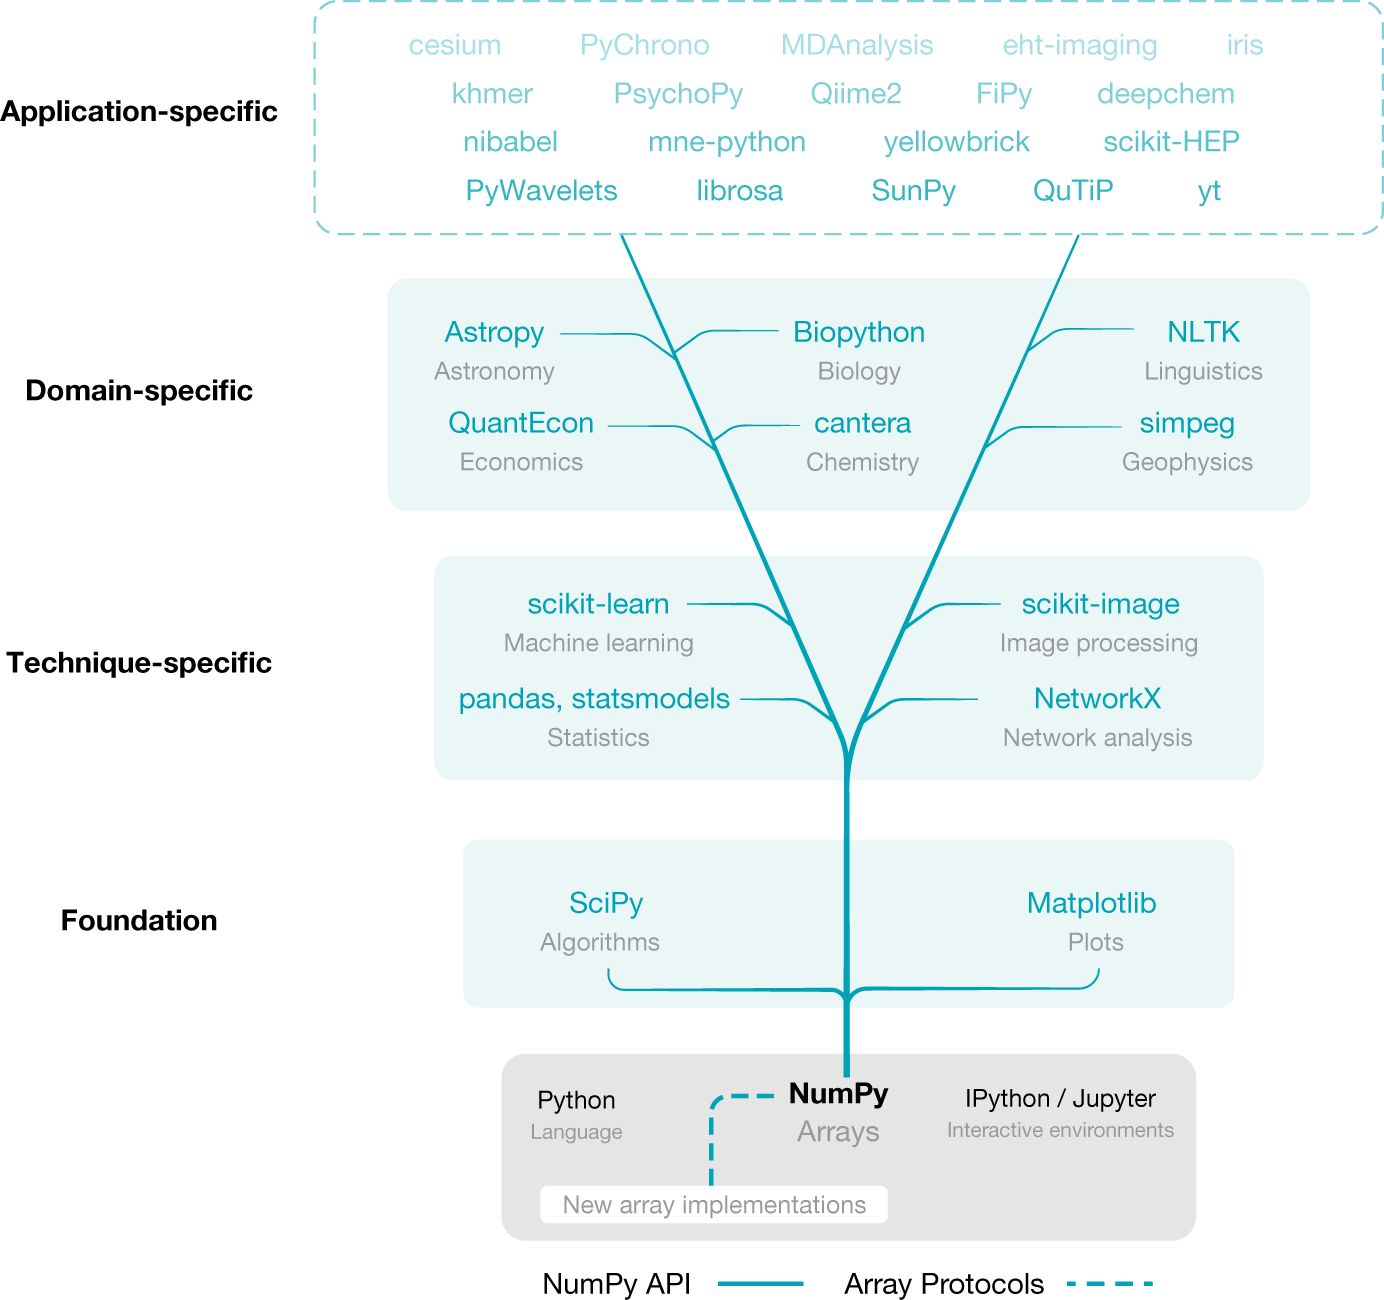
\includegraphics[keepaspectratio]{images/41586_2020_2649_Fig2_HTML.png}}
\caption{Figure~2.1: La librairie NumPy est le fondement de nombreuses
librairies scientifiques (d'après
{(\href{references.html\#ref-NumpyNature}{Harris 2020})}).}
\end{figure}

\subsubsection{\texorpdfstring{{2.3.2} Information de
base}{2.3.2 Information de base}}\label{information-de-base}

Les deux informations de base à afficher sur une matrice sont 1) les
dimensions de la matrice et 2) le format de stockage (le type). Pour
cela, on peut utiliser le (\hyperref[lst-numpyshape]{bloc~{2.6}}), le
résultat nous informe que la matrice a 3 dimensions et une taille de
\texttt{(442,\ 553,\ 3)} et un type \texttt{uint8} qui représente 1
octet (8 bit). Par conséquent, la matrice a \texttt{442} lignes,
\texttt{553} colonnes et \texttt{3} canaux ou bandes. Il faut prêter une
attention particulière aux valeurs minimales et maximales tolérées par
le type de la donnée comme indiqué dans le
(\hyperref[tbl-numpytype]{tableau~{2.1}}) (voir aussi
\href{https://numpy.org/doc/stable/user/basics.types.html}{Data types
--- NumPy v2.1 Manual}).

\phantomsection\label{0b232cfc}
\phantomsection\label{lst-numpyshape}
\begin{figure}
\centering
\phantomsection\label{lst-numpyshape}
\begin{Shaded}
\begin{Highlighting}[]
\ImportTok{import}\NormalTok{ cv2}
\NormalTok{img }\OperatorTok{=}\NormalTok{ cv2.imread(}\StringTok{\textquotesingle{}modis{-}aqua.PNG\textquotesingle{}}\NormalTok{)}
\BuiltInTok{print}\NormalTok{(}\StringTok{\textquotesingle{}Nombre de dimensions: \textquotesingle{}}\NormalTok{,img.ndim)}
\BuiltInTok{print}\NormalTok{(}\StringTok{\textquotesingle{}Dimensions de la matrice: \textquotesingle{}}\NormalTok{,img.shape)}
\BuiltInTok{print}\NormalTok{(}\StringTok{\textquotesingle{}Type de la donnée: \textquotesingle{}}\NormalTok{,img.dtype)}
\end{Highlighting}
\end{Shaded}
\caption{Bloc de code~2.6: Lecture d'une image en format PNG avec
OpenCV}
\end{figure}

\begin{verbatim}
Nombre de dimensions:  3
Dimensions de la matrice:  (442, 553, 3)
Type de la donnée:  uint8
\end{verbatim}

\phantomsection\label{tbl-numpytype}
\begin{longtable}[]{@{}llrrr@{}}
\toprule\noalign{}
dtype & Nom & Taille (bits) & Min & Max \\
\midrule\noalign{}
\endhead
\bottomrule\noalign{}
\endlastfoot
uint8 & char & 8 & 0 & 255 \\
int8 & signed char & 8 & -127 & 128 \\
uint16 & unsigned short & 16 & 0 & -32768 \\
int16 & short & 16 & 0 & 655355 \\
\end{longtable}

\subsubsection{\texorpdfstring{{2.3.3} Découpage et indexation de la
matrice}{2.3.3 Découpage et indexation de la matrice}}\label{duxe9coupage-et-indexation-de-la-matrice}

L'indexation et le découpage (\emph{slicing}) des matrices dans NumPy
sont des techniques essentielles pour manipuler efficacement les données
multidimensionnelles en Python, offrant une syntaxe puissante et
flexible pour accéder et modifier des sous-ensembles spécifiques
d'éléments dans les tableaux (voir
\hyperref[fig-naturenumpy2]{figure~{2.2}}). Indexer une matrice consiste
à accéder à une valeur dans la matrice pour une position particulière,
la syntaxe générale est \texttt{matrice{[}ligne,\ colonne,\ bande{]}} et
est similaire à la manipulation des
\href{https://docs.python.org/fr/3/tutorial/introduction.html\#lists}{listes}
en Python. Les indices commencent à \texttt{0} et se termine à la
\texttt{taille-1} de l'axe considéré.

\phantomsection\label{fig-naturenumpy2}
\begin{figure}
\centering
\pandocbounded{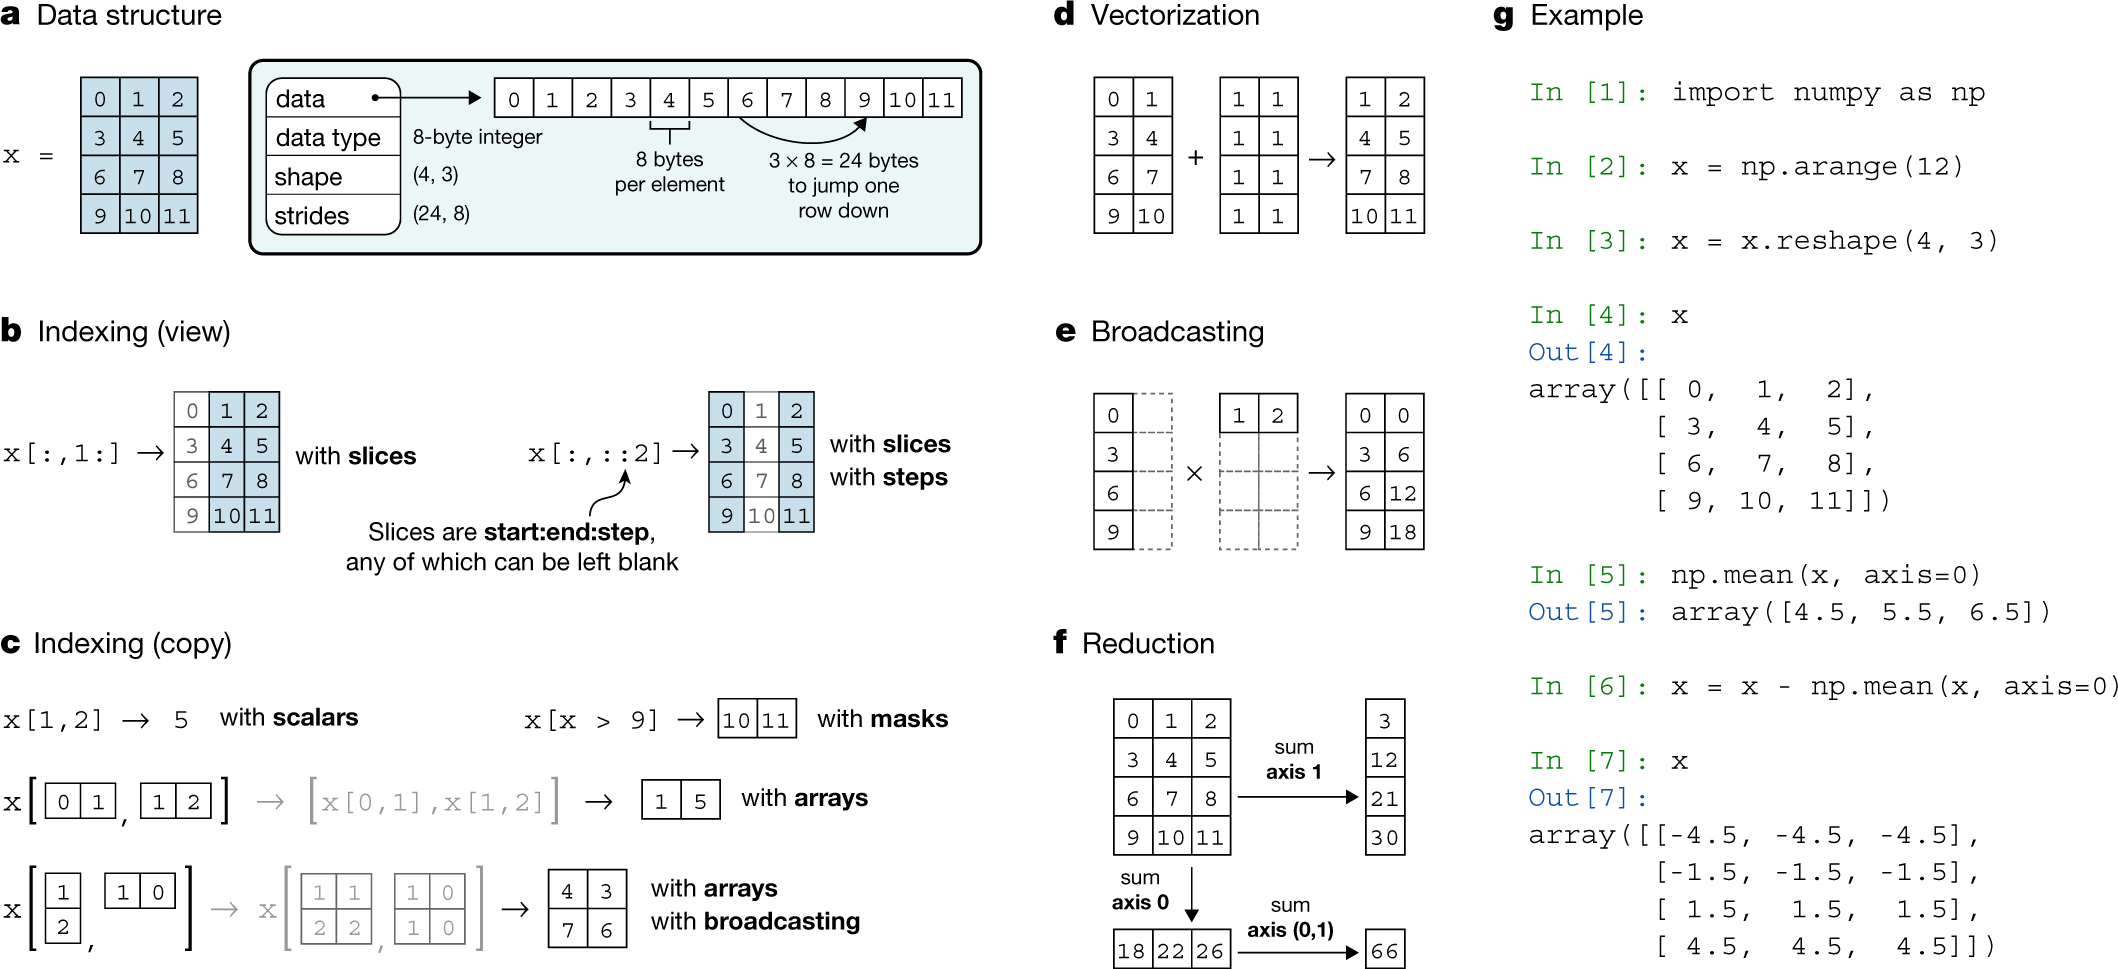
\includegraphics[keepaspectratio]{images/41586_2020_2649_Fig1_HTML.png}}
\caption{Figure~2.2: Vue d'ensemble des opérations de base des matrices
avec NumPy}
\end{figure}

Le découpage (ou \emph{slicing} en anglais) consiste à produire une
nouvelle matrice qui est un sous-ensemble de la matrice d'origine. Un
découpage se fait avec le symbole `:', la syntaxe générale pour définir
un découpage est \texttt{{[}début:fin:pas{]}}. Si on ne spécifie pas
\texttt{début} ou \texttt{fin} alors les valeurs 0 ou
\texttt{dimension-1} sont considérées implicitement. Quelques exemples:
* choisir un pixel en particulier avec toutes les bandes:
\texttt{matrice{[}1,1,:{]}} * choisir la colonne 2:
\texttt{matrice{[}:,2,:{]}}

La syntaxe de base pour le découpage (\emph{slicing}) des tableaux NumPy
repose sur l'utilisation des deux-points (\texttt{:}) à l'intérieur des
crochets d'indexation. Cette notation permet de sélectionner des plages
d'éléments de manière concise et intuitive. La structure générale du
découpage est \texttt{matrice{[}start:stop:step{]}}, où : 1.
\texttt{start} représente l'index de départ (inclus) 2. \texttt{stop}
indique l'index de fin (exclu) 3. \texttt{step} définit l'intervalle
entre chaque élément sélectionné

Si l'un de ces paramètres est omis, NumPy utilise des valeurs par défaut
: 0 pour \texttt{start}, la taille du tableau pour \texttt{stop}, et 1
pour \texttt{step}. Par exemple, pour un tableau unidimensionnel
\texttt{array}, on peut extraire les éléments du deuxième au quatrième
avec \texttt{array{[}1:4{]}}. Pour sélectionner tous les éléments à
partir du troisième, on utiliserait \texttt{array{[}2:{]}}. Cette
syntaxe s'applique également aux tableaux multidimensionnels, où chaque
dimension est séparée par une virgule. Ainsi, pour une matrice 2D m,
\texttt{m{[}0:2,\ 1:3{]}} sélectionnerait une sous-matrice 2x2 composée
des deux premières lignes et des deuxième et troisième colonnes.
L'indexation négative est également supportée, permettant de compter à
partir de la fin du tableau. Par exemple, \texttt{a{[}-3:{]}}
sélectionnerait les trois derniers éléments d'un tableau.

\phantomsection\label{b3549f48}
\phantomsection\label{cb10}
\begin{Shaded}
\begin{Highlighting}[]
\ImportTok{import}\NormalTok{ cv2}
\NormalTok{img }\OperatorTok{=}\NormalTok{ cv2.imread(}\StringTok{\textquotesingle{}modis{-}aqua.PNG\textquotesingle{}}\NormalTok{)}
\NormalTok{img\_col }\OperatorTok{=}\NormalTok{ img[:,}\DecValTok{1}\NormalTok{,:]}
\BuiltInTok{print}\NormalTok{(}\StringTok{\textquotesingle{}Nombre de dimensions: \textquotesingle{}}\NormalTok{,img\_col.ndim)}
\BuiltInTok{print}\NormalTok{(}\StringTok{\textquotesingle{}Dimensions de la matrice: \textquotesingle{}}\NormalTok{,img\_col.shape)}
\end{Highlighting}
\end{Shaded}

\begin{verbatim}
Nombre de dimensions:  2
Dimensions de la matrice:  (442, 3)
\end{verbatim}

\textbf{Une vue versus une copie}

Avec NumPy, les manipulations peuvent créer des vues ou des copies. Une
vue est une simple représentation de la même donnée originale alors
qu'une copie est un nouvel espace mémoire.

Par défaut, un découpage créé une vue.

On peut vérifier si l'espace mémoire est partagé avec
\texttt{np.shares\_memory(arr,\ slice\_arr)}.

On peut toujours forcer une copie avec la méthode \texttt{copy()}

\paragraph{\texorpdfstring{{2.3.3.1}
Masquage}{2.3.3.1 Masquage}}\label{masquage}

L'utilisation d'un masque est un outil important en traitement d'image
car la plupart des images de télédétection contiennent des pixels non
valides qu'il faut exclure des traitements (ce que l'on appelle le
\emph{no data} en Anglais). Il y a plusieurs raison possibles pour la
présence de pixels non valides:

\begin{enumerate}
\def\labelenumi{\arabic{enumi}.}
\item
  L'image est projetée dans une grille cartographique et certaines
  zones, généralement situées en dehors de l'empreinte au sol du
  capteur, sont à exclure.
\item
  La présence de nuages que l'on veut exclure.
\item
  La présence de pixels erronés dûs à des problèmes de capteurs.
\item
  La présence de valeurs non numériques (\emph{not a number} ou
  \texttt{nan})
\end{enumerate}

La librairie NumPy fournit des mécanismes pour exclure automatiquement
certaines valeurs.

\subsubsection{\texorpdfstring{{2.3.4} Changement de projection
cartographique}{2.3.4 Changement de projection cartographique}}\label{changement-de-projection-cartographique}

\subsection{\texorpdfstring{{2.4} Données en
géoscience}{2.4 Données en géoscience}}\label{donnuxe9es-en-guxe9oscience}

Les données en géoscience contiennent beaucoup de métadonnées et peuvent
être composées de différentes variables avec différentes unités,
résolution, etc. Ces données sont aussi souvent étiquetées avec des
dates sur certains axes, des coordonnées géographiques, des identifiants
d'expériences, etc. Par conséquent, utiliser seulement des matrices est
souvent incomplet {(\href{references.html\#ref-xarray-2017}{Hoyer et
Hamman 2017})}.

Calibration, unités, données manquantes, données éparses.

\subsubsection{\texorpdfstring{{2.4.1}
xarray}{2.4.1 xarray}}\label{xarray}

\href{https://docs.xarray.dev/en/latest/getting-started-guide/why-xarray.html}{Xarray}
est une puissante bibliothèque Python qui améliore les matrices
multidimensionnelles de type numpy en y ajoutant des étiquettes, des
dimensions, des coordonnées et des attributs. Elle fournit deux
structures de données principales : \texttt{DataArray} (un tableau
étiqueté à N dimensions) et \texttt{Dataset} (une base de données de
tableaux multidimensionnels en mémoire).

Les caractéristiques principales sont les suivantes:

\begin{itemize}
\item
  Opérations sur les dimensions nommées au lieu des numéros d'axe
\item
  Sélection et opérations basées sur les étiquettes
\item
  Diffusion automatique de tableaux basée sur les noms de dimensions
\item
  Alignement de type base de données avec des étiquettes de coordonnées
\item
  Suivi des métadonnées grâce aux dictionnaires Python
\end{itemize}

\paragraph{\texorpdfstring{{2.4.1.1}
Avantages}{2.4.1.1 Avantages}}\label{avantages}

La bibliothèque réduit considérablement la complexité du code et
améliore la lisibilité du code pour les applications de calcul
scientifique dans divers domaines, notamment la physique, l'astronomie,
les géosciences, la bio-informatique, l'ingénierie, la finance et
l'apprentissage profond. Elle s'intègre de manière transparente avec
NumPy et pandas tout en restant compatible avec l'écosystème Python au
sens large.

\paragraph{\texorpdfstring{{2.4.1.2}
DataArray}{2.4.1.2 DataArray}}\label{dataarray}

Un tableau multidimensionnel étiqueté avec des propriétés clées :

\begin{itemize}
\item
  \texttt{valeurs} : Les données réelles du tableau
\item
  \texttt{dims} : Dimensions nommées (par exemple, « x », « y », « z »)
\item
  \texttt{coords} : Dictionnaire de tableaux étiquetant chaque point
\item
  \texttt{attrs} : Stockage de métadonnées arbitraires
\item
  \texttt{name} : Identifiant facultatif
\end{itemize}

\paragraph{\texorpdfstring{{2.4.1.3}
Dataset}{2.4.1.3 Dataset}}\label{dataset}

Un conteneur de type dictionnaire de \texttt{DataArrays} avec des
dimensions alignées, contenant :

\begin{itemize}
\item
  \texttt{dims} : Dictionnaire de correspondance entre les noms des
  dimensions et les longueurs
\item
  \texttt{data\_vars} : Dictionnaire des variables du DataArray
\item
  \texttt{coords} : Dictionnaire des variables de coordonnées
\item
  \texttt{attrs} : Stockage des métadonnées
\end{itemize}

Les principales différences sont les suivantes :

\begin{itemize}
\item
  \texttt{DataArray} contient un seul tableau avec des étiquettes
\item
  Le \texttt{Dataset} contient plusieurs DataArrays alignés.
\end{itemize}

Ces trois structures prennent en charge les opérations de type
dictionnaire et les calculs de coordination tout en conservant les
métadonnées.

\phantomsection\label{fig-xarray}
\begin{figure}
\centering
\pandocbounded{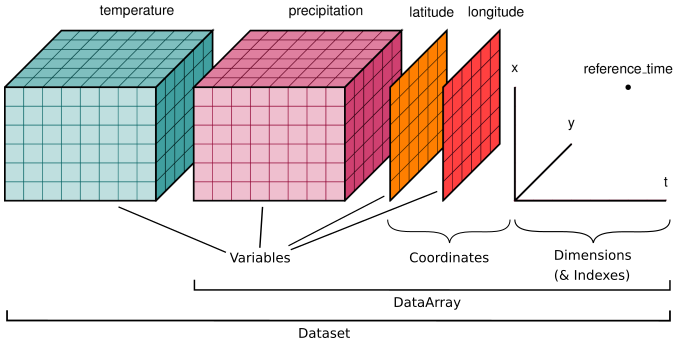
\includegraphics[keepaspectratio]{images/xarray-dataset-diagram.png}}
\caption{Figure~2.3: Organisation d'un Dataset dans xarray}
\end{figure}

\phantomsection\label{refs}
\begin{CSLReferences}{1}{0}
\bibitem[\citeproctext]{ref-NumpyNature}
Harris, Millman, C. R. 2020. {«~Array programming with NumPy.~»}
\emph{{Nature}}: 357‑362.
\url{https://doi.org/10.1038/s41586-020-2649-2}.

\bibitem[\citeproctext]{ref-xarray-2017}
Hoyer, S. et J. Hamman. 2017. {«~xarray: N-D labeled Arrays and Datasets
in Python.~»} \emph{{Journal of Open Research Software}} 5 (1): 10.
\url{https://doi.org/10.5334/jors.148}.

\bibitem[\citeproctext]{ref-OGCGeoTIFF}
OGC. 2019. {«~{OGC GeoTIFF Standard}.~»}
\url{https://docs.ogc.org/is/19-008r4/19-008r4.html/}.

\end{CSLReferences}

\end{document}
